\documentclass{article}
\usepackage{float}
\usepackage{graphicx}
\begin{document}

\title{SBMS6002}
\author{Yu-ping Lin}
\maketitle

\section{introudction}
Computer and the internet play the most conspicuous roles in all aspects of human life and have altered the way we gather, collect, and analyze information from individuals or specific groups of people online. Bioinformatics is not an exception in the profit. Bioinformatics is an interdisciplinary research field that utilizes mathematical or statistical methods and computer programming to analyze and interpret biological data, due to the digitalization of relevant processes and availability of high throughput devices, the volume, variety, velocity, and variety of data is increasing with a great pace. The explosion of available biological data is tremendously supported by the advent of next-generation sequencing technologies. Several reported had mentioned that the Next Generation Sequencing(NGS) platforms use nanopore sequencing has generating piles of biological data faster and at a considerably lower cost. The cost and the time to sequence a genome is approximately following Moore's low trajectory in the decade before 2008, but the recent breakthrough in sequencing technologies results in costs drop dramatically than would be expected by Moore’s law. For instance, in the earlier time, the estimated cost for sequencing a human genome was a three billion project requiring longer waiting times. Today, personal genomes can be  sequence and mapped in a few days at an affordable price. 



As the cost of data generation continues to decrease, 
research members are able to generate gigantic amount of sequence data rapidly, in order to extract hidden valued information, which is beneficial across every branch of scientist to make the critical decision of whether it is genomics or proteomics or metabolomics or personalized medicine. For example, Personal genomics contains much valuable information and is a  key enabler for predictive medicine and personalized medicine, where a patient's genome profile will enable scientists to determine the most appropriate medical treatment and in turn minimizing drug side effects and accelerating the curing process. 

Thus the voluminous increase in data,has in turn placed a high demand in the development of compatible hardware and software forstorage, processing and retrieval of information from huge databases where the data can be redundant or unstructured. 





\begin{figure}[H]
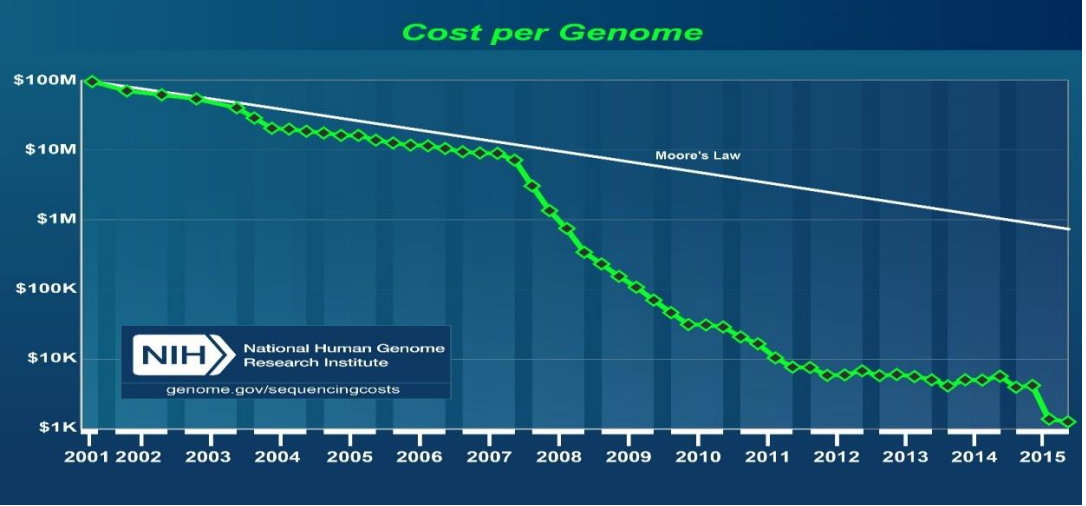
\includegraphics[width=0.9 \columnwidth]{/Users/yu-pinglin/Desktop/Essay/6002.png}
\centering
\caption{Changes in the cost of sequencing over time}
\end{figure}







\bibliography{ref}
\bibliographystyle{plain}
\end{document}
